
\chapter{Introducción}

Un sistema fotovoltaico es el conjunto de equipos eléctricos y electrónicos
que producen energía eléctrica a partir de la radiación solar. El
principal componente de este sistema es el módulo fotovoltaico, a
su vez compuesto por células capaces de transformar la energía luminosa
incidente en energía eléctrica de corriente continua. El resto de
equipos incluidos en un sistema fotovoltaico depende en gran medida
de la aplicación a la que está destinado. A grandes rasgos los sistemas
fotovoltaicos pueden clasificarse en tres grandes grupos (figura \ref{fig:ClasificacionAplicaciones}):
conectados a red (\emph{grid connected}), autónomos (\emph{off-grid})
y de bombeo.

%
\begin{figure}


\begin{centering}
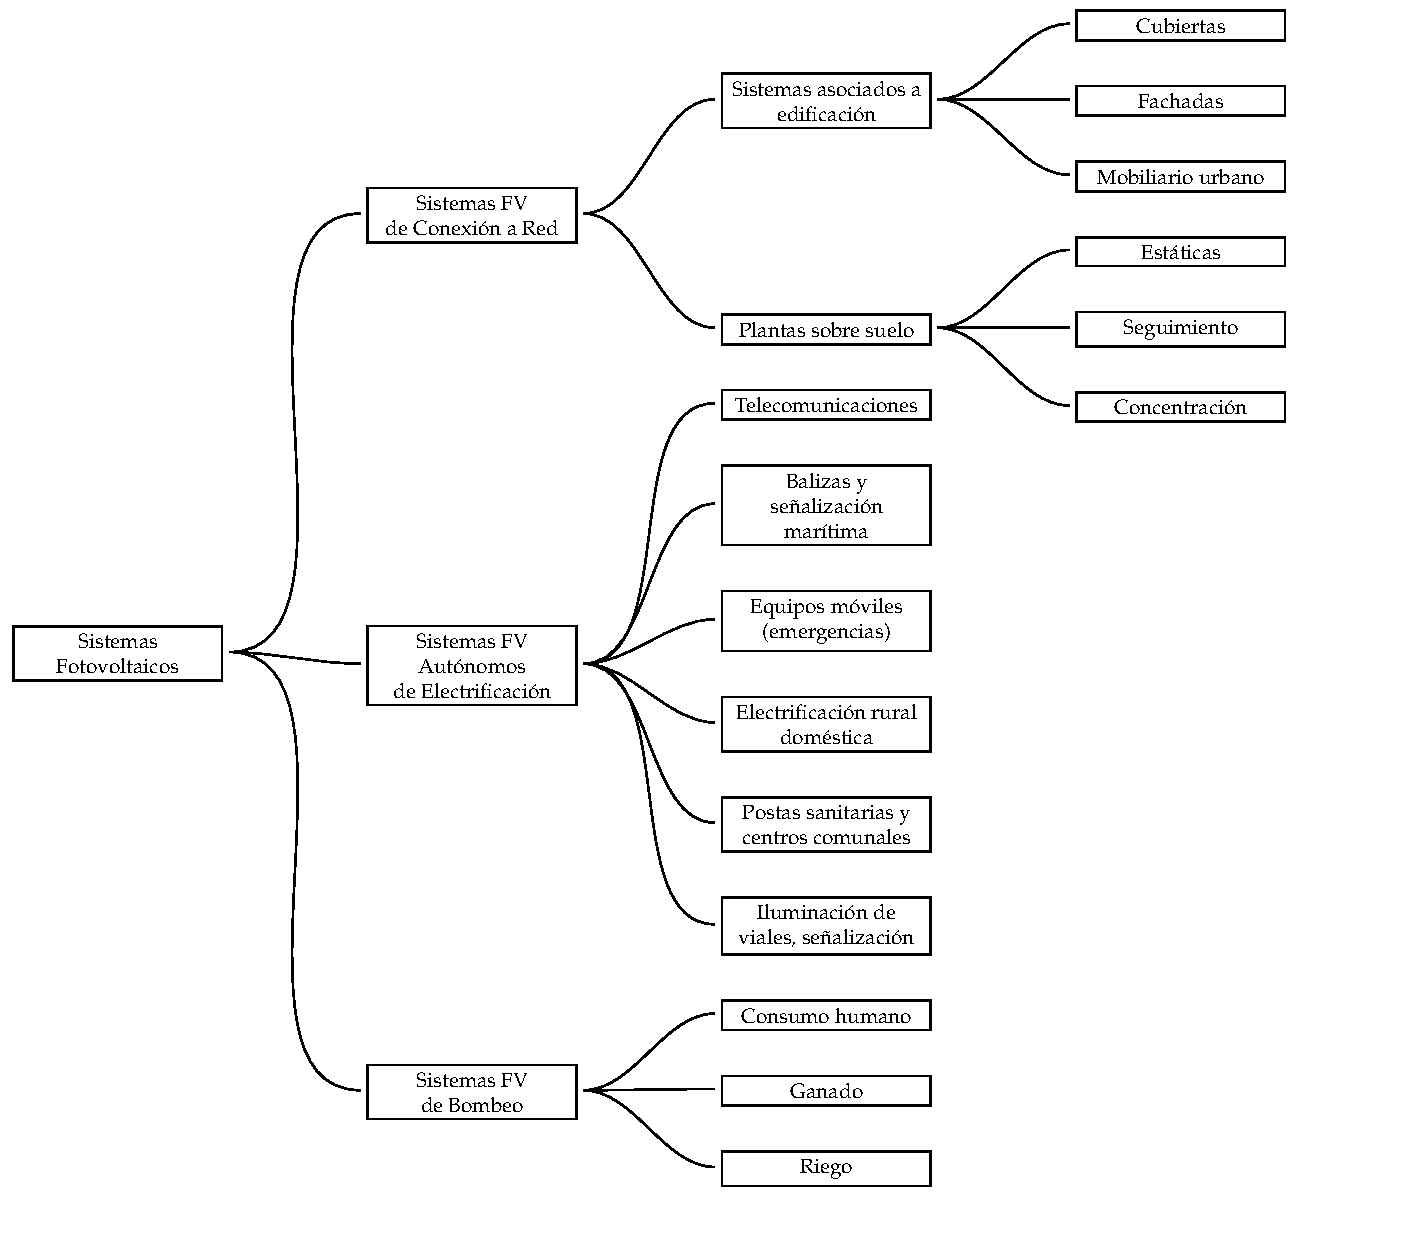
\includegraphics[scale=0.8]{../figs/ClasificacionSistemas}\caption{Clasificación de aplicaciones fotovoltaicas.\label{fig:ClasificacionAplicaciones}}

\end{centering}


\end{figure}


Los sistemas conectados a red (capítulo \ref{cha:SFCR}) producen
energía eléctrica para ser inyectada íntegramente en la red convencional.
Dado que no deben satisfacer ninguna demanda de consumo de forma directa
ni garantizar el mismo, no necesitan incorporar equipos de acumulación
de energía. Para permitir el correcto acoplamiento con la red eléctrica
estos sistemas incorporan un equipo inversor que adecúa la potencia
producida por el generador fotovoltaico a las condiciones de la red
convencional. Estos sistemas pueden a su vez ser divididos en sistemas
instalados sobre suelo y sistemas en edificación. Los sistemas sobre
suelo (figura \ref{fig:SistemaSobreSuelo}), concebidos exclusivamente
para producir energía y obtener el rendimiento económico asociado,
suelen superar los $\SI{100}{\kilo\watt}$ de potencia. Los sistemas
en edificación (figura \ref{fig:SistemaEdificacion}) abarcan funciones
adicionales a la producción de energía, tales como sustitución de
componentes arquitectónicos, efecto estético, sombreado de acristalamientos,
etc. En general, son sistemas más pequeños que los instalados sobre
suelo, normalmente de potencias inferiores a los $\SI{100}{\kilo\watt}$.

%
\begin{figure}
\hfill{}\subfloat[Sistema conectado a red instalado sobre suelo.\label{fig:SistemaSobreSuelo}]{\begin{centering}
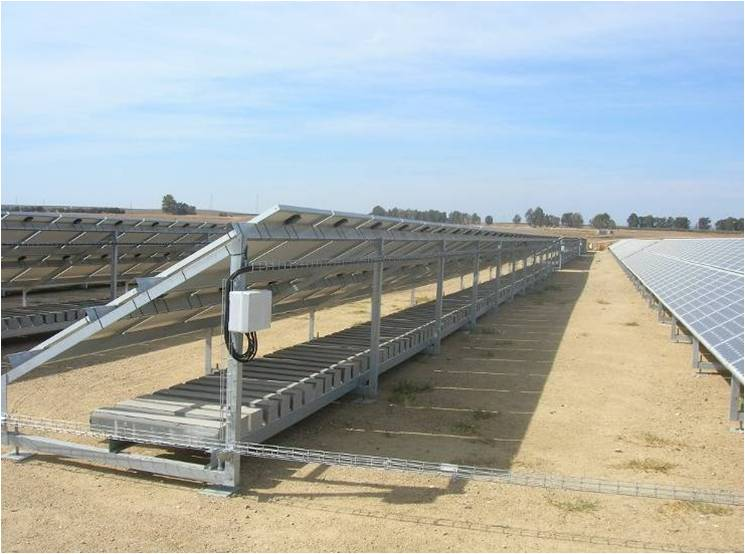
\includegraphics[scale=0.25]{../figs/EstructuraEstaticaSuelo}
\par\end{centering}

}\hfill{}\subfloat[Sistema conectado a red instalado como acristalamiento de un edificio.\label{fig:SistemaEdificacion}]{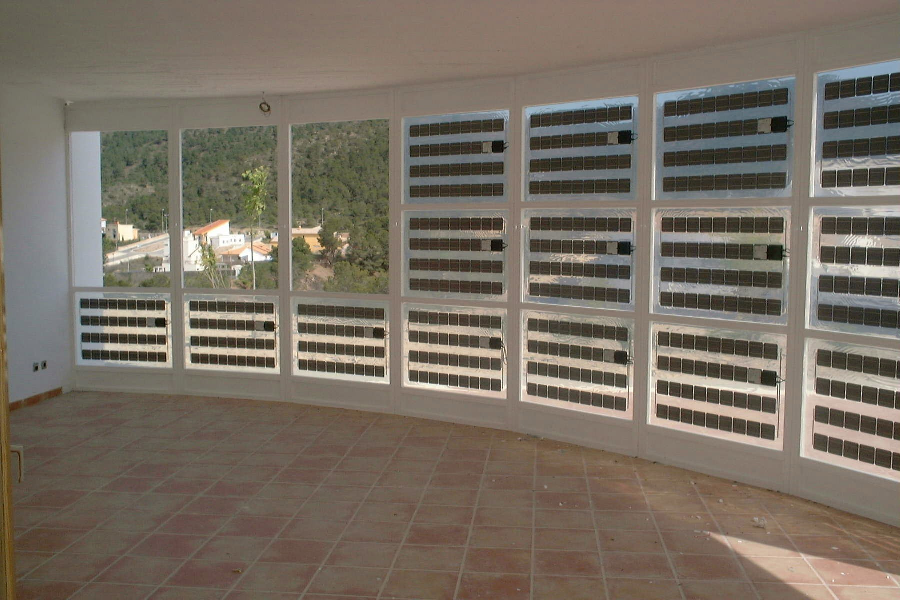
\includegraphics[scale=0.46]{../figs/Torreguil}

}\hfill{}

\caption{Sistemas fotovoltaicos conectados a red.}



\end{figure}


Los sistemas autónomos (capítulo \ref{cha:Sistemas-Fotovoltaicos-Autonomos})
abarcan una variedad muy amplia de aplicaciones. Su denominador común
es la necesidad de satisfacer una demanda energética determinada.
Por esta razón, prácticamente todos los sistemas autónomos incorporan
un equipo de acumulación de energía. Estos sistemas pueden ser clasificados
en tres grupos por razón de su aplicación asociada: profesionales,
electrificación rural y pequeño consumo. 

Dentro de las aplicaciones de pequeño consumo se emplean pequeños
módulos fotovoltaicos, frecuentemente de silicio amorfo, alimentando
equipos electrónicos como calculadoras o relojes, cargadores de móviles,
pequeñas herramientas eléctricas, balizas domésticas, etc. 

Las aplicaciones profesionales son variadas y abarcan campos tales
como los radioenlaces (figura \ref{fig:SistemaRadioenlace}), la protección
catódica de gasoductos, hoteles, señales de tráfico y navegación aérea,
refrigeración de vacunas, equipos remotos de adquisición y transmisión
de datos, e incluso alimentación equipos espaciales como satélites.
Todas estas aplicaciones se caracterizan por requerir una fiabilidad
muy elevada. Dado que el corte de suministro en estas aplicaciones
tiene consecuencias de elevado coste, suele optarse por incorporar
un generador fotovoltaico y un acumulador electroquímico de tamaño
superior al estrictamente necesario y así reducir al mínimo la probabilidad
de fallo. En algunos casos se opta por incorporar un grupo electrógeno,
ya sea para reducir el tamaño del acumulador o para funcionar como
equipo de socorro.

%
\begin{figure}
\begin{centering}
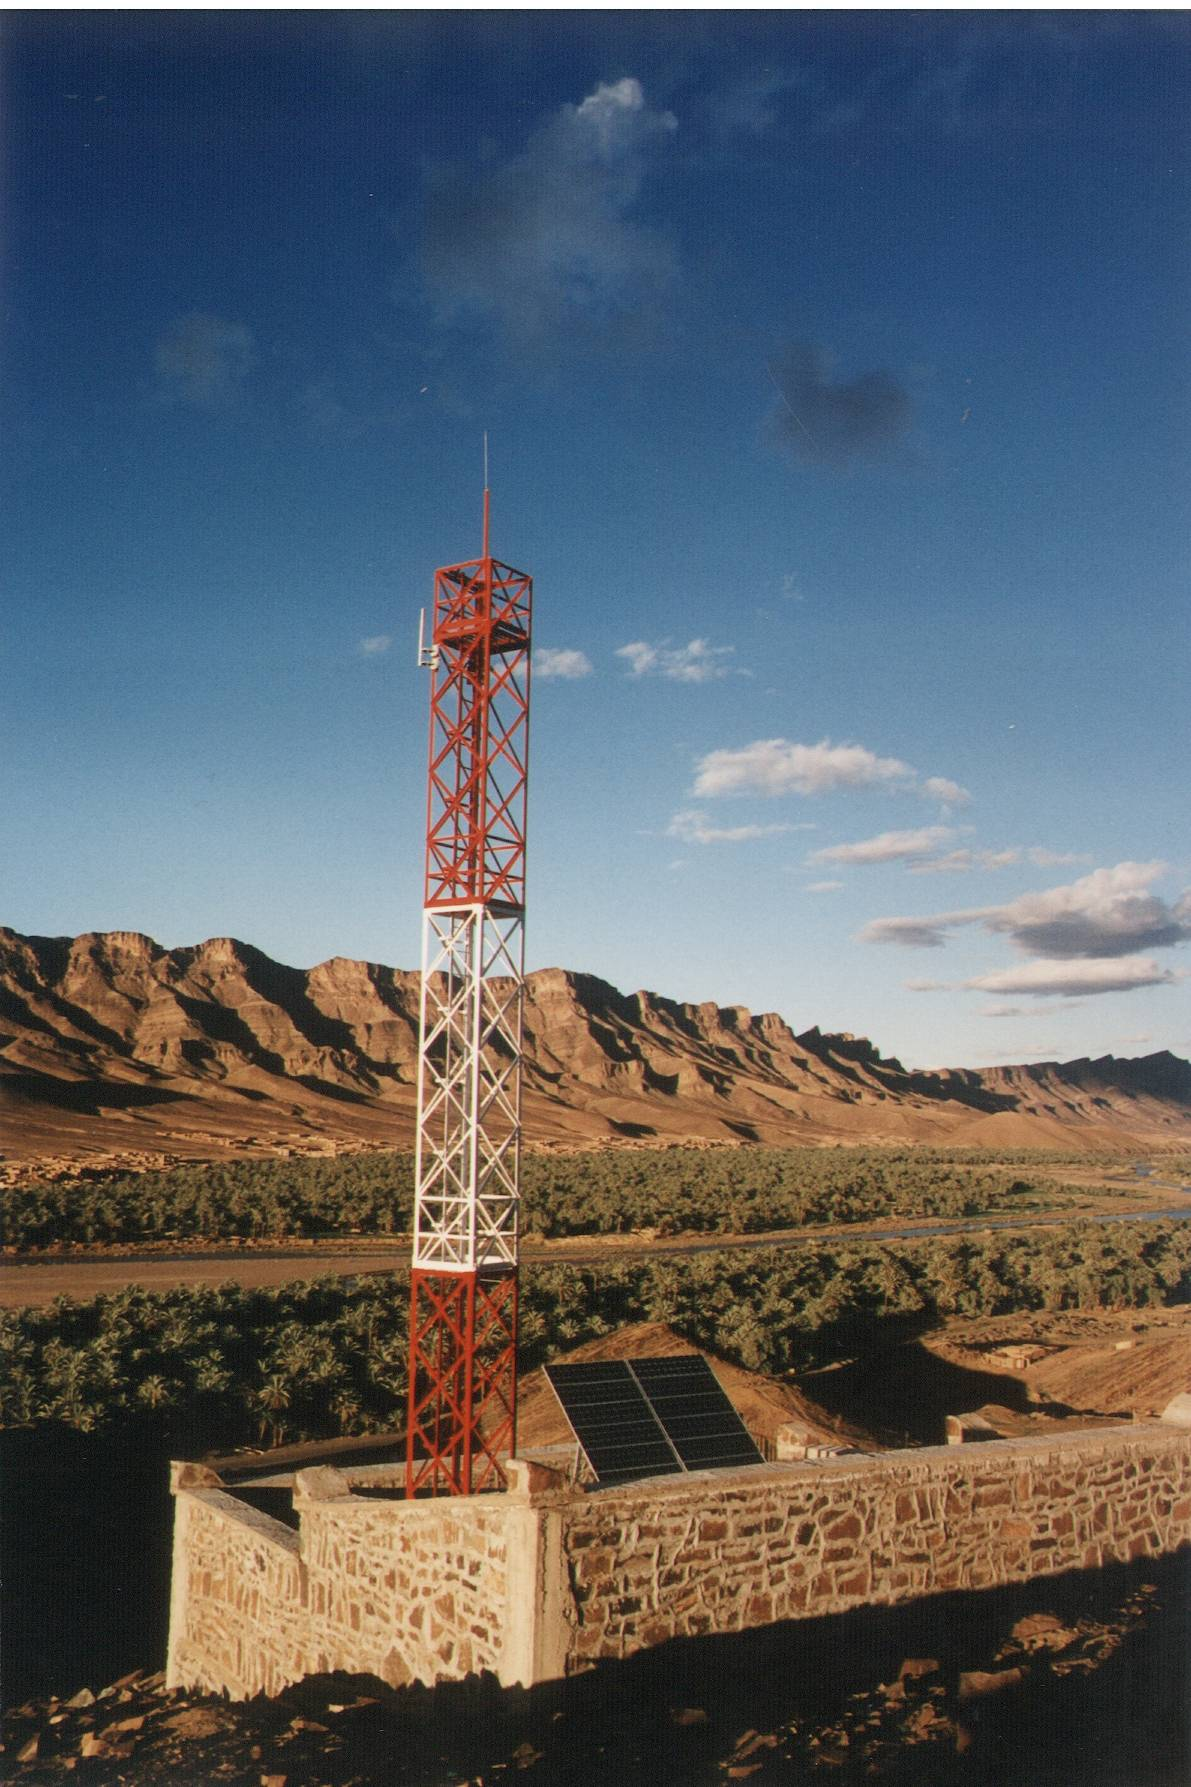
\includegraphics[scale=0.6]{../figs/TelefoniaRural}
\end{centering}

\caption{Sistema fotovoltaico autónomo alimentando un radioenlace.\label{fig:SistemaRadioenlace}}

\end{figure}


Los sistemas de electrificación rural suministran energía eléctrica
a poblaciones rurales alejadas de redes eléctricas convencionales.
Son sistemas frecuentemente englobados en programas de cooperación
al desarrollo, financiados por ONG's u organismos como el Banco Mundial
o la Unión Europea. Dentro de los sistemas de electrificación rural
predominan los sistemas domésticos (\emph{solar home systems, SHS}),
las centrales híbridas y los sistemas de bombeo. Tanto los sistemas
domésticos como las centrales híbridas (ambos estudiados en el capítulo
\ref{cha:Sistemas-Fotovoltaicos-Autonomos}) proporcionan energía
para alimentar equipos de iluminación, radio, televisión y pequeñas
herramientas eléctricas. 

Los sistemas domésticos (figura \ref{fig:SHS}),
habitualmente con potencias de $\SI{100}{\watt}$ o $\SI{200}{\watt}$,
están asociados a una vivienda familiar y en algunos casos a centros
comunales o centros de salud. 

Las centrales híbridas, compuestas por
un generador fotovoltaico, un acumulador electroquímico y un grupo
electrógeno o turbina eólica, proveen una red eléctrica para un poblado
rural. El tamaño de estas centrales depende del tamaño de la población
asociada, con potencias que van desde los $\SI{10}{\kilo\watt}$ hasta
los $\SI{100}{\kilo\watt}$. 

Los sistemas de bombeo (capítulo \ref{cha:SFB})
 emplean la energía eléctrica que produce el generador fotovoltaico
para accionar una motobomba que eleva y transporta agua desde un acuífero
hasta un depósito (figura \ref{fig:Sistema-de-bombeo}) o una red
de distribución. Para reducir costes y aumentar la fiabilidad, en
estos sistemas es frecuente acumular la energía en forma de energía
potencial del agua almacenada en el depósito elevado. Las aplicaciones
de los sistemas de bombeo incluyen el suministro de agua para consumo
humano o animal, el riego de plantaciones individuales o comunitarias
y la desalinización del agua extraída con sistemas de ósmosis inversa.

%
\begin{figure}
\subfloat[Sistema doméstico.\label{fig:SHS}]{\begin{centering}
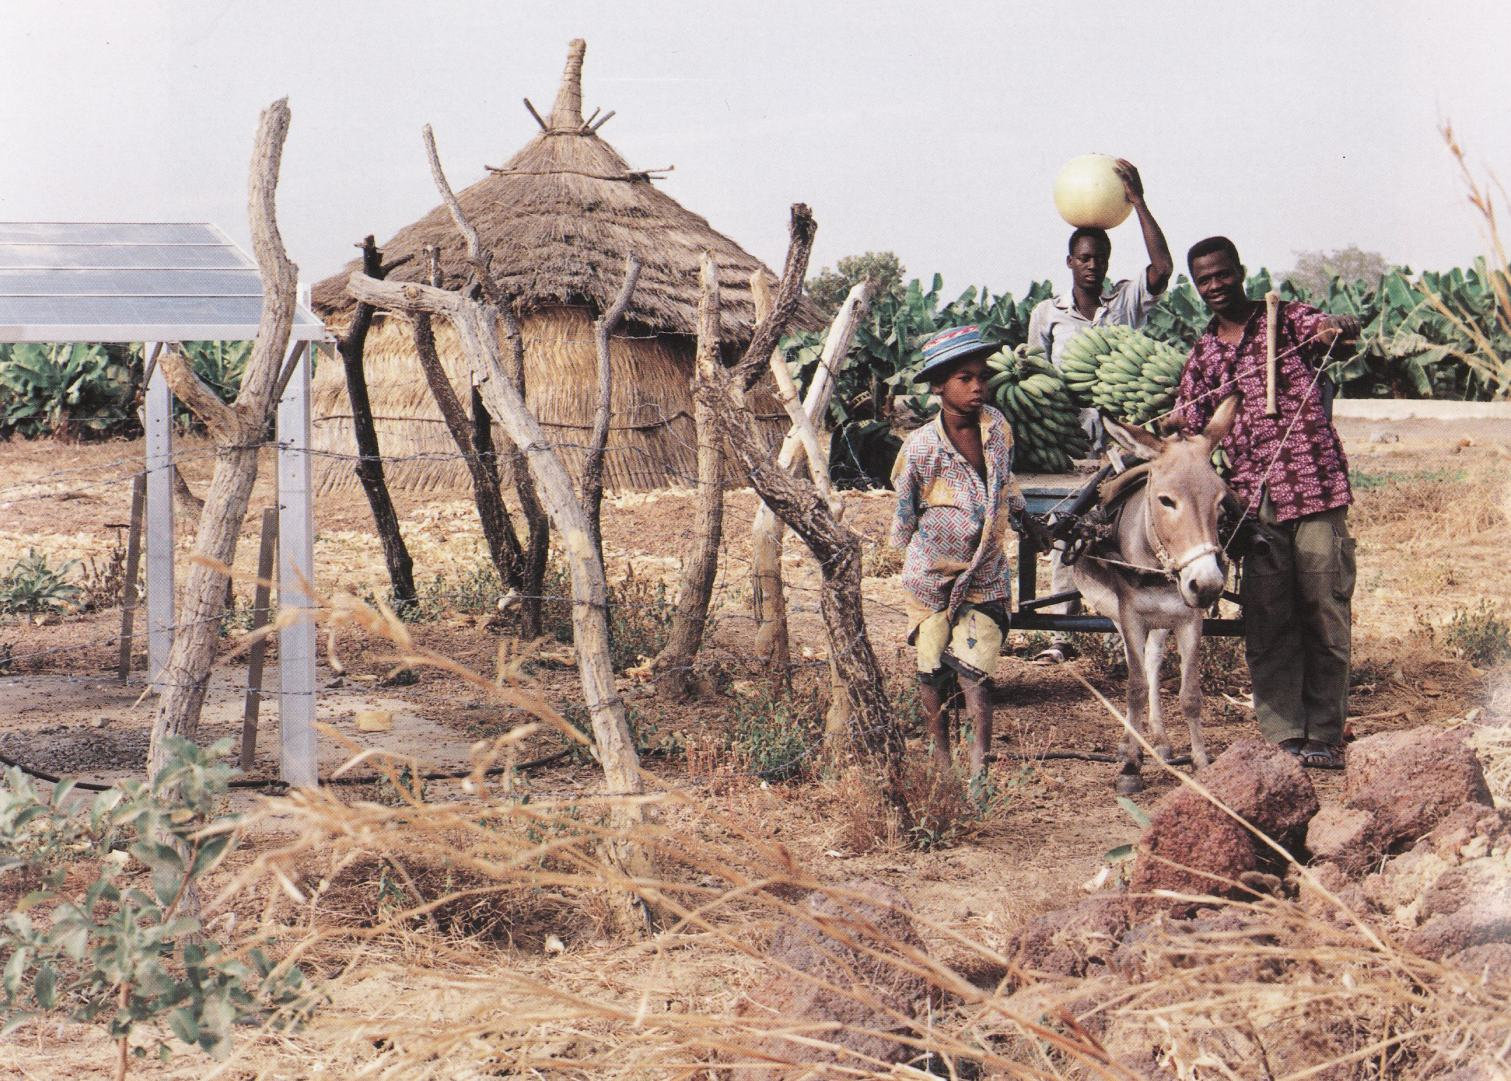
\includegraphics[scale=0.73]{../figs/er}
\par\end{centering}

}\subfloat[Sistema de bombeo con depósito elevado.\label{fig:Sistema-de-bombeo}]{\begin{centering}
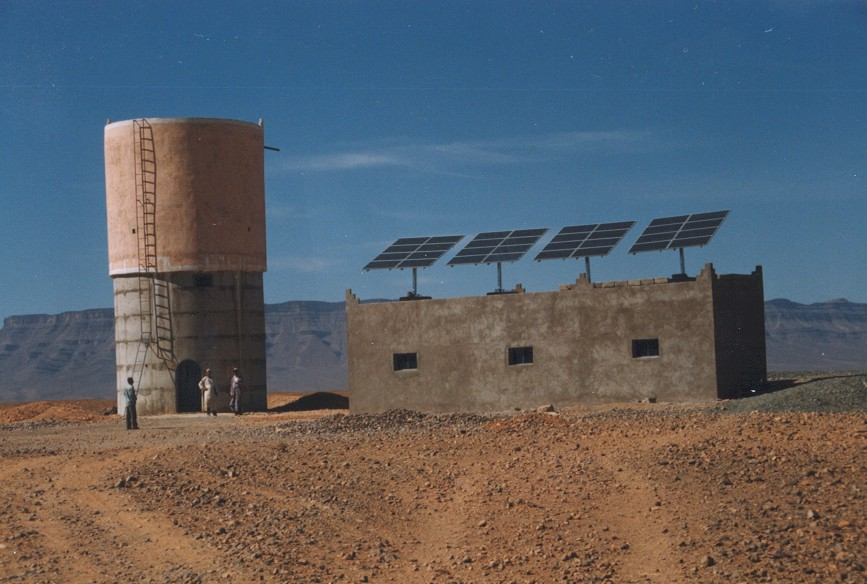
\includegraphics[scale=0.28]{../figs/Bombeo}
\par\end{centering}

}

\caption{Sistemas fotovoltaicos autónomos de electrificación rural.}



\end{figure}


Según el informe \emph{Global Market Outlook for Photovoltaics until
2016} de la \emph{European Photovoltaics Industry Association}
\cite{EPIA2012} la potencia fotovoltaica instalada en el planeta
al finalizar el 2011 era superior a los 69 GW. Europa es la región
que lidera el sector, con más de 51 GW instalados en 2011, lo que
representa alrededor del 75\% de la potencia total mundial. A
continuación destacan Japón con 5 GW, Estados Unidos con 4.4 GW, y
China con 3.1 GW. A pesar de que es muy difícil establecer
cifras fiables de la potencia instalada en sistemas autónomos, no
hay duda de que una proporción muy alta se debe a sistemas conectados
a red. 

%%% Local Variables:
%%% mode: LaTex
%%% TeX-master: "ESF.tex"
%%% End: 